
\exer{Percolation}
\setcounter{numques}{0}
\section{Présentation}
%\begin{multicols}{2}
Pour ce TP, on utilisera le fichier \texttt{Percolation\_Sujet.py}

La percolation \footnote{du latin \emph{percolare} : couler à travers.} désigne le passage d'un fluide à
travers un solide poreux. Ce terme fait bien entendu référence au café 
produit par le passage de l'eau à travers une poudre de café comprimée,
mais dans un sens plus large peut aussi bien s'appliquer à
l'infiltration des eaux de pluie jusqu'aux nappes phréatiques ou encore
à la propagation des feux de forêt par contact entre les feuillages des
arbres voisins.

L'étude scientifique des modèles de percolation s'est développée à
partir du milieu du XXe siècle et touche aujourd'hui de nombreuses
disciplines, allant des mathématiques à l'économie en passant par la
physique et la géologie.

%\setcounter{section}{1}
\section{Choix d'un modèle}\label{choix-dun-modele}


Nous allons aborder certains phénomènes propres à la percolation par
l'intermédiaire du modèle suivant : une grille carrée $n\times n$,
chaque case pouvant être aléatoirement ouverte ou fermée.
%ouverte (avec une probabilité $p$) ou fermée (avec une probabilité $1-p$). 
La question à laquelle nous
allons essayer de répondre est la suivante : est-il possible de joindre
le haut et le bas de la grille par une succession de cases ouvertes
adjacentes ?

\begin{figure}[H]
\begin{center}

\includegraphics[width=.7\linewidth]{illustration_perco.jpg}
\caption{Deux exemples de grilles $10\times10$. La percolation
n'est possible que dans le second cas (les cases ouvertes sont les cases
blanches). \label{fig1}}
\end{center}
\end{figure}



\subsection*{Création et visualisation de grilles}


La grille de percolation sera représentée par le type \texttt{list}. Cette grille sera elle-même composée de \texttt{n} listes de \texttt{n} flottants (tableau $n\times n$). 
Une fois la grille \texttt{grille} créée, la case d'indice $(i, j)$ est référencée par \texttt{grille[i][j]}.

Si la case \texttt{grille[i][j]} est vide on lui affectera la valeur 0 (case ouverte, le fluide peut passer). Si la case \texttt{grille[i][j]} empêche le fluide de passer, on lui affectera la valeur 1 (case fermée). 

\vspace{.25cm}

\question{Implémenter la fonction \texttt{creation\_grille\_vierge(n:int) -> list} permettant de créer un tableau de \texttt{n} lignes,  \texttt{n} colonnes de 0. On utilisera pour cela deux boucles \texttt{for} imbriquées. }

L'instruction  \texttt{creation\_grille\_vierge(3)} renverra le résultat suivant \texttt{[[0, 0, 0], [0, 0, 0], [0, 0, 0]]}.

\vspace{.25cm}

On dispose de la fonction \texttt{afficher\_grille(grille : list) -> None} permettant d'afficher une grille. 


\question{Donner les instructions permettant d'afficher une grille vierge de taille 3.}

\question{Afficher la grille suivante \texttt{[[1, 0, 1], [0, 1, 0], [1, 0, 1]]}.}

\question{Implémenter la fonction \texttt{creation\_zebreh(n:int) -> list} permettant de créer une grille constituée de bandes horizontales noires puis blanches. \texttt{creation\_zebreh(3)} renverra \texttt{[[1, 1, 1], [0, 0, 0], [1, 1, 1]]}. Valider votre résultat en utilisant la fonction \texttt{afficher\_grille}.}

\question{Implémenter la fonction \texttt{creation\_zebrev(n:int) -> list} permettant de créer une grille constituée de bandes verticales noires puis blanches. \texttt{creation\_zebrev(3)} renverra \texttt{[[1, 0, 1], [1, 0, 1], [1, 0, 1]]}. Valider votre résultat en utilisant la fonction \texttt{afficher\_grille}.}

\question{Implémenter la fonction \texttt{creation\_damier(n:int) -> list} permettant de créer une grille en forme de damier. \texttt{creation\_damier(3)} renverra \texttt{[[1, 0, 1], [0, 1, 0], [1, 0, 1]]}. Valider votre résultat en utilisant la fonction \texttt{afficher\_grille}.}





%
%Les deux modules essentiels dont nous aurons besoin sont les modules
%\texttt{numpy} (manipulation de tableaux bi-dimensionnels) et \texttt{matplotlib.pyplot}
%(graphisme), qu'il convient d'importer :
%
%\begin{lstlisting}
%import numpy as np
%import matplotlib.pyplot as plt
%\end{lstlisting}
%
%Nous aurons aussi besoin de la fonction \textbf{\texttt{rand}} du module \texttt{numpy.random}
%(fonction qui retourne un nombre pseudo- aléatoire de l'intervalle
%$\left[0,1\right[$ et accessoirement de la fonction \texttt{ListedColormap} du
%module \texttt{matplotlib.colors} (pour choisir l'échelle chromatique à utiliser
%pour la représentation graphique). Ces deux fonctions seront importées
%directement, puisque nous n'aurons pas besoin des modules entiers :
%
%\begin{lstlisting}
%from numpy.random import rand
%from matplotlib.colors import ListedColormap
%\end{lstlisting}
%
%La grille de percolation sera représentée par le type \texttt{np.array}. La
%fonction \texttt{np.zeros((n, p))} renvoie un tableau de $n$ lignes et
%$p$ colonnes contenant dans chacune de ses cases le nombre flottant
%0.0. Une fois un tableau \texttt{tab} créé, la case d'indice $(i, j)$ est
%référencée indifféremment par \texttt{tab[i][j]} ou par \texttt{tab[i,j]} et
%peut être lue et modifiée (comme d'habitude, les indices débutent à 0).
%Enfin, on notera que si tab est un tableau, l'attribut \texttt{tab.shape}
%retourne le couple $(n, p)$ de ses dimensions verticale et
%horizontale (le nombre de lignes et de colonnes, \texttt{tab} étant vu comme une
%matrice).
%
%Dans la suite de ce document, on représentera une grille de percolation
%par un tableau $n\times n$, les cases fermées contenant le nombre
%flottant $0.0$ et les cases ouvertes le nombre flottant $1.0$.


On va maintenant créer une grille pour simuler la percolation. 
Afin de remplir la grille, on dispose de la fonction \texttt{rand()} de la bibliothèque \texttt{random} permettant de renvoyer un nombre aléatoire compris dans l'intervalle $\verb![!0,1\verb![!$.

On souhaite remplir une grille de taille \texttt{n} de la façon suivante : 
\begin{itemize}
\item l'utilisateur choisit un nombre \texttt{p} compris entre 0 et 1 via un paramètre d'une fonction ;
\item création d'une grille vide de taille \texttt{n};
\item pour chaque élément de la grille :
\begin{itemize}
\item on génère un nombre aléatoire \texttt{nb} compris dans l'intervalle $\verb![!0,1\verb![!$ ;
\item si \texttt{nb>p} alors l'élément est remplacé par la valeur 1. 
\end{itemize}
\end{itemize}


Ainsi, si \texttt{p} vaut 1, la case aura 100\,\% de chance d'être ouverte. Si \texttt{p} vaut 0,25, la case aura 25\,\% de chance d'être ouverte.


\question{Définir une fonction de signature \texttt{def creation\_grille(p: float, n: int) -> list} à deux paramètres : un nombre réel $p$ (qu'on supposera dans l'intervalle $\verb![!0,1\verb!]!$) et un entier naturel $n$, qui renvoie un tableau $(n,n)$ dans lequel chaque case sera ouverte (valeur 0) avec la probabilité $p$ et fermée sinon (valeur~1). }



%\subsubsection*{Visualisation de la grille}
%
%Pour visualiser simplement la grille, nous allons utiliser la fonction
%\texttt{plt.matshow} : appliquée à un tableau, celle-ci présente ce dernier sous
%forme de cases colorées en fonction de leur valeur.
%
%Les couleurs sont choisies en fonction d'une échelle chromatique que
%vous pouvez visualiser à l'aide de la fonction plt.colorbar(). Celle
%utilisée par défaut va du bleu au rouge ; puisque nos grilles ne
%contiennent pour l'instant que les valeurs 0 ou 1, les cases fermées
%apparaîtrons en bleu, et les cases ouvertes, en rouge.
%%
%
%\subsubsection*{Changer l'échelle chromatique}
%
%L'argument par défaut \texttt{cmap} de la fonction \texttt{plt.matshow} permet de modifier
%l'échelle chromatique utilisée. La fonction \texttt{ListedColormap} va nous
%permettre de créer l'échelle de notre choix. Puisque nous n'aurons que
%trois états possibles (une case pleine représentée par la valeur $0.0$),
%une case vide représentée par la valeur $1.0$ et plus tard une case
%remplie d'eau représentée par la valeur $0.5$) une échelle à trois
%couleurs suffit. Vous pouvez utiliser celle-ci :
%
%\begin{lstlisting}
%echelle = ListedColormap(['black', 'aqua', 'white'])
%\end{lstlisting}
%
%
%
%\question{Écrire une fonction \texttt{afficher\_grille(grille,nom\_de\_fichier)} 
%qui prend en argument une variable grille qui correspond à une grille de 
%percolation générée précédemment et ne renvoyant rien mais enregistrant dans 
%\texttt{nom\_de\_fichier} le graphe obtenu. On pourra exporter une grille de
% $10\times 10$ cases avec l'échelle suggérée précédemment, l'enregistrer sous 
% le nom \texttt{tp09\_q02\_vos\_noms.png} et l'envoyer à votre professeur.}
%
%

%\end{quote}
%
\section{Percolation}\label{percolation}
%




Une fois la grille créée, les cases ouvertes de la première ligne sont
remplies par un fluide, ce qui sera représenté par la valeur $2$ dans
les cases correspondantes. Le fluide pourra ensuite être diffusé à
chacune des cases ouvertes voisines d'une case contenant déjà le fluide jusqu'à remplir toutes les cases ouvertes possibles.


\begin{figure}[H]
\begin{center}
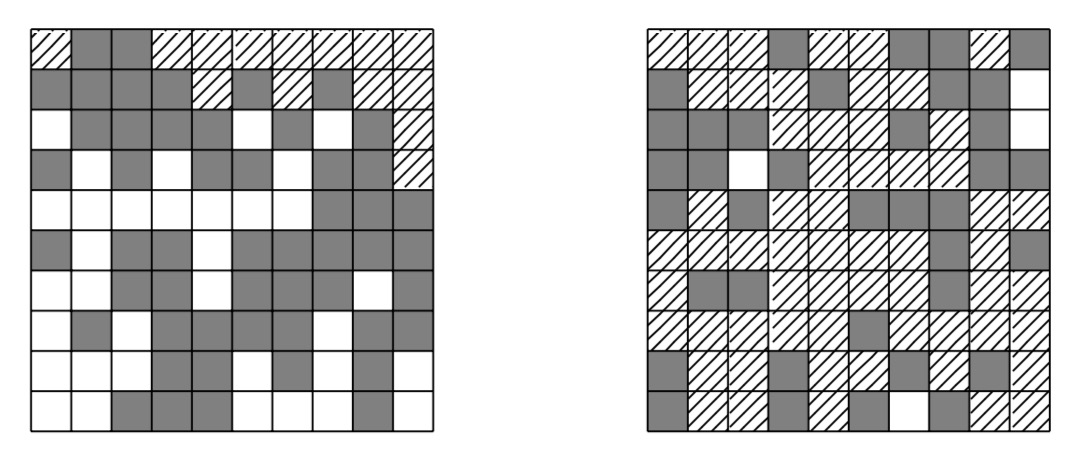
\includegraphics[width=0.6\textwidth]{illustration_perco2}
\caption{les deux grilles de la figure \ref{fig1}, une fois le processus de percolation terminé (le fluide est représenté par des hachures)\label{fig2}.}
\end{center}
\end{figure}

\subsection{Percolation << naïve >>}

Dans un premier temps, nous allons créer une fonction intermédiaire permettant de savoir si, pour une case de coordonnées \texttt{[i,j]} de la grille, un de ses voisins est rempli (valeur 2) ou non. 

\question{Écrire une fonction \texttt{a\_un\_voisin\_rempli(grille:list,i:int,j:int) -> bool} retournant \texttt{True} si un des voisins est rempli, \texttt{False} si aucun des voisins n'est rempli.}

\question{Écrire une fonction \texttt{percolation(grille : list) -> None} qui prend en argument une
grille et qui remplit de fluide celle-ci, en appliquant l'algorithme
exposé ci-dessous :}
\textit{
\begin{itemize}
\item pour la première ligne, si la case est ouverte on la remplit (passage de la valeur \texttt{0} à la valeur \texttt{2});
\item pour les cases des lignes suivantes : si la case est ouverte et qu'un voisin est rempli, alors on remplit cette case.
\end{itemize}}

\question{En affichant la grille avant et après percolation avec différentes valeurs de \texttt{p}, visualiser que l'algorithme ne répond pas complètement à la problématique. Modifier la fonction précédente en conséquence.}
\subsection{Percolation un peu plus évoluée -- Facultatif}


\question{Écrire une fonction \texttt{percolation(grille : list) -> None} qui prend en argument une
grille et qui remplit de fluide celle-ci, en appliquant l'algorithme
exposé ci-dessous :
\begin{enumerate}
\item Créer une liste contenant initialement les coordonnées des cases ouvertes de la première ligne de la grille et remplir ces cases de liquide.
\item  Puis, tant que cette liste n'est pas vide, effectuer les opérations suivantes :
  \begin{enumerate}
  \item extraire de cette liste les coordonnées d'une case quelconque ;
  \item ajouter à la liste les coordonnées des cases voisines qui sont encore vides, et les remplir de liquide.
  \end{enumerate}
\end{enumerate}
L'algorithme se termine quand la liste est vide.}


\subsection{Validation de la percolation}


\question{Rédiger un script vous permettant de visualiser une grille avant et
après remplissage, et faire l'expérience avec quelques valeurs de
$p$ pour une grille de taille raisonnable (commencer avec $n
= 10$ pour vérifier visuellement que votre algorithme est correct, puis
augmenter la taille de la grille, par exemple avec $n = 64$). On pourra l'exporter et l'enregistrer sous le nom  \texttt{tp\_n\_q03\_vos\_noms.png}.}



On dit que la percolation est réussie lorsqu'à la fin du processus au
moins une des cases de la dernière ligne est remplie du fluide.

\question{Écrire une fonction \texttt{teste\_percolation(p : float, n : int) -> bool} qui prend en argument
un réel $p\in\left[0,1\right]$ et un entier $n\in \mathbb{N}^*$, crée une grille, effectue la percolation et
renvoie : }
\begin{itemize}
\item \texttt{True} lorsque la percolation est réussie, c'est-à-dire lorsque le bas
  de la grille est atteint par le fluide ;
\item \texttt{False} dans le cas contraire.
\end{itemize}

\newpage
%
\section{Seuil critique}\label{seuil-critique}
%
%\begin{quote}
Nous allons désormais travailler avec des grilles de taille $128\times 128$ \footnote{Baisser cette valeur si le temps de calcul sur votre ordinateur est trop long.}


Faire quelques essais de percolation avec différentes valeurs de $p$. Vous observerez assez vite qu'il semble exister un seuil $p_0$ en deçà duquel la percolation
échoue presque à chaque fois, et au delà duquel celle-ci réussit presque
à chaque fois. Plus précisément, il est possible de montrer que pour une
grille de taille infinie, il existe un seuil critique
$p_0$ en deçà duquel la percolation échoue toujours,
et au delà duquel la percolation réussit toujours. Bien évidemment, plus
la grille est grande, plus le comportement de la percolation tend à se
rapprocher du cas de la grille théorique infinie.
\begin{figure}[H]
\centering
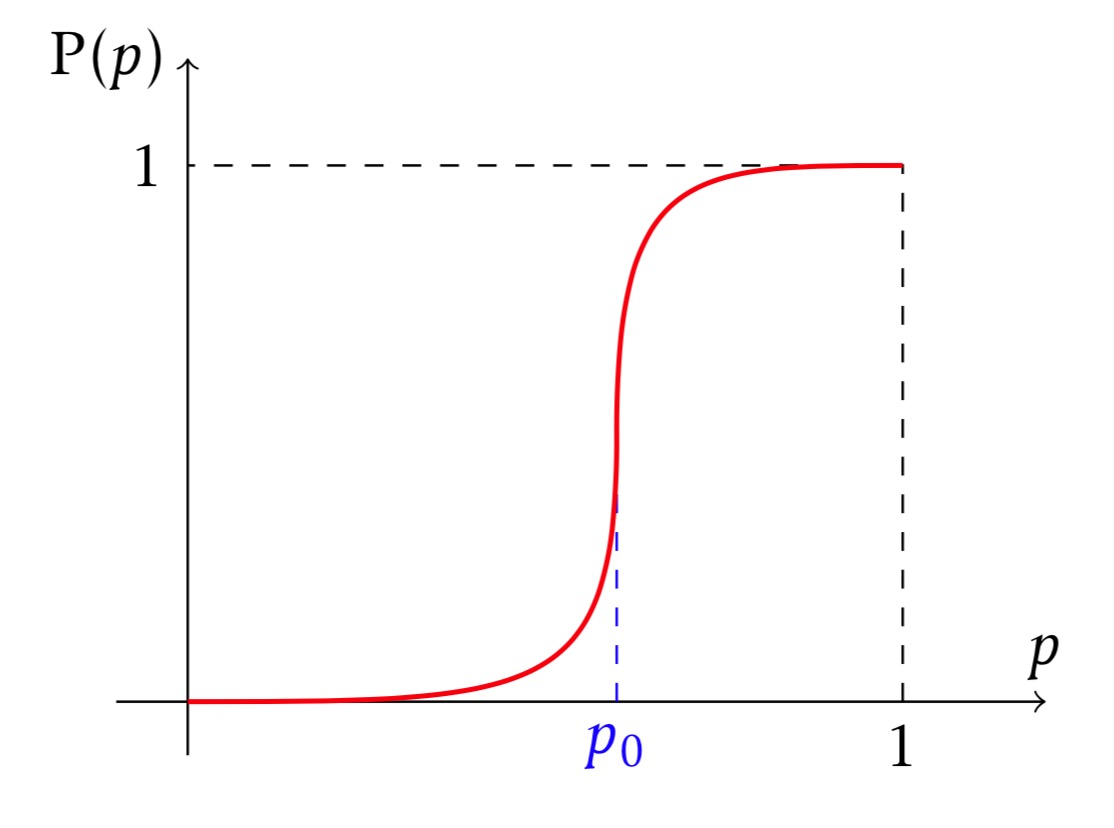
\includegraphics[width=0.4\linewidth]{proba}
\caption{L'allure théorique du graphe de la fonction $P(p)$ \label{fig3}.}
\end{figure}

%L'allure théorique du graphe de la fonction P(p)

Notons $P(p)$ la probabilité pour le fluide de traverser la grille. Pour déterminer une valeur approchée de la probabilité de traverser la grille, on se contente d'effectuer $k$ essais pour une valeur de $p$ puis de renvoyer le nombre moyen de fois où le test de percolation est vérifié.\\

\question{Rédiger la fonction \texttt{proba(p : float, k : int, n : int) -> float} qui prend en argument le nombre d'essai $k$, la variable $p$ ainsi que le nombre de cases $n$ sur la largeur de la grille et qui renvoie $P(p)$.}



%\question{Écrire une fonction \texttt{tracer\_proba(n : int ,nom\_de\_fichier : str) -> None}
%qui prend en argument une taille $n$ ne renvoyant rien mais enregistrant 
%dans \texttt{nom\_de\_fichier} le graphe obtenu. On pourra traiter le 
%cas d'une grille de $128\times 128$ cases et enregistrer la figure obtenue 
%sous le nom \texttt{tp\_n\_q06\_vos\_noms.png}.} 

La fonction suivante prend en argument une taille $n$ et affiche le graphe obtenu. On pourra traiter le 
cas d'une grille de $128\times 128$ cases.% et visualiser la figure obtenue.
%sous le nom \texttt{tp\_n\_q06\_vos\_noms.png}.

\begin{lstlisting}
import numpy as np
import matplotlib.pyplot as plt
#Q06
def tracer_proba(n):
    x=np.linspace(0,1,21)
    y=[]
    for p in x:
        y.append(proba(p,20,n))
    plt.clf()
    plt.plot(x,y)
    plt.show()
    return None
\end{lstlisting}

%
%P(\emph{p})
%\end{quote}
%
%1
%
%\begin{quote}
%\emph{p}
%
%\emph{p}0 1
%
%Figure 3 -- \emph{L'allure théorique du graphe de la fonction} P\emph{.}
%\end{quote}
%
%
%Pour déterminer le seuil critique $p_0$, on peut procéder à une recherche dichotomique (assez grossière) en convenant que si
%$P(p) < 0,4$ alors $p < p_0$ et si $P(p) > 0,6$ alors $p > p_0$
%\question{ (Facultative) En utilisant une recherche dichotomique, chercher à estimer le plus précisément possible la valeur numérique du seuil $p_0$.}
%\end{enumerate}
%
%\section{Propriétés
%macroscopiques}\label{propriuxe9tuxe9s-macroscopiques}
%
%\begin{quote}
%A l'instar de la thermodynamique, on peut décrire le comportement d'un
%système lors d'une transition de phase en introduisant des propriétés
%macroscopiques. Dans le cas de la percolation, on peut par exemple
%définir la densité moyenne \emph{d}(\emph{p}) de cases ouvertes
%atteintes par le fluide.
%
%Question 5.
%\end{quote}
%
%\begin{enumerate}
%\def\labelenumi{\alph{enumi})}
%\item
%  Définir une fonction densite qui prend en argument une grille dans
%  laquelle la percolation a eu lieu et qui retourne la valeur de sa
%  densité.
%\item
%  À l'aide d'un nombre raisonnable d'échantillons, définir alors la
%  fonction d qui à une probabilité \emph{p} ∈ {[}0\emph{,} 1{[} associe
%  la densité moyenne de la percolation dans une grille 128 × 128.
%\item
%  Tracer le graphe de \emph{d}(\emph{p}) pour \emph{p} ∈ {[}0\emph{,}
%  1{[}.
%\end{enumerate}
%
%\section{Et pour les plus rapides}\label{et-pour-les-plus-rapides}
%
%\begin{quote}
%Recommencez toute cette étude, mais cette fois-ci avec une grille
%hexagonale. Il est possible de prouver que pour une grille hexagonale
%carrée le seuil critique \emph{p}\textsubscript{0} est exactement égal à
%\emph{p}\textsubscript{0} = 1\emph{/}2 ; le vérifier expérimentalement
%et chercher à le démontrer (en utilisant un argument de symétrie).
%\end{quote}

%\end{multicols}



\end{document}
